\documentclass[11pt]{article}
\usepackage{amsmath, amsthm, amssymb,lscape, natbib,epstopdf,
	cases, bbm, indentfirst}
\usepackage{amsfonts}
\usepackage{graphicx}
\usepackage{epstopdf}
\usepackage{colortbl}
\usepackage[hang,small,bf]{caption}
\usepackage{setspace}
\usepackage{amsmath}
\usepackage[nohead]{geometry}
\usepackage[bottom]{footmisc}
\usepackage{endnotes}
\usepackage{rotating}
\usepackage{xr}
\usepackage{xr-hyper}
\usepackage[backref = section]{hyperref}
\usepackage[section]{placeins}
\allowdisplaybreaks

\definecolor{citec}{rgb}{0,0,.5}
\definecolor{linkc}{rgb}{0,0,.6}
\definecolor{bcolor}{rgb}{1,1,1}

\hypersetup{
	colorlinks = true,
	urlcolor=linkc,
	linkcolor=linkc,
	citecolor = citec,
	filecolor = linkc,
	pdfauthor={Pat Moran}}

\usepackage{pstricks}
\usepackage{pstcol}

\onehalfspacing

%\input{tcilatex}
\geometry{left=1in,right=1.25in,top=1in,bottom=1in}
\interfootnotelinepenalty=10000

\begin{document}


	%-------------------------------------------------
	\title{Household spending, leisure and well-being in retirement}
	\date{}
	\maketitle

A big area of controversy in economics is how households adjust their consumption and leisure decisions as they approach and enter into retirement. Previous research has documented significant drops in households' spending at retirement, which potentially indicates that they have under-saved in preparation for old age and therefore suffer a fall in living standards. However, other papers have suggested that, as the opportunity cost of leisure falls at retirement, households optimally switch leisure for consumption and therefore falls in spending do not reflect drops in living standards. This project aims to document the extent to which these changes in spending and time use differ across different types of households, and ultimately, to understand what drives these difference.

\section{Life Cycle Consumption Dynamics (APC)}


\begin{figure}[h]
	% \caption{Life Cycle Consumption}
	\centering
	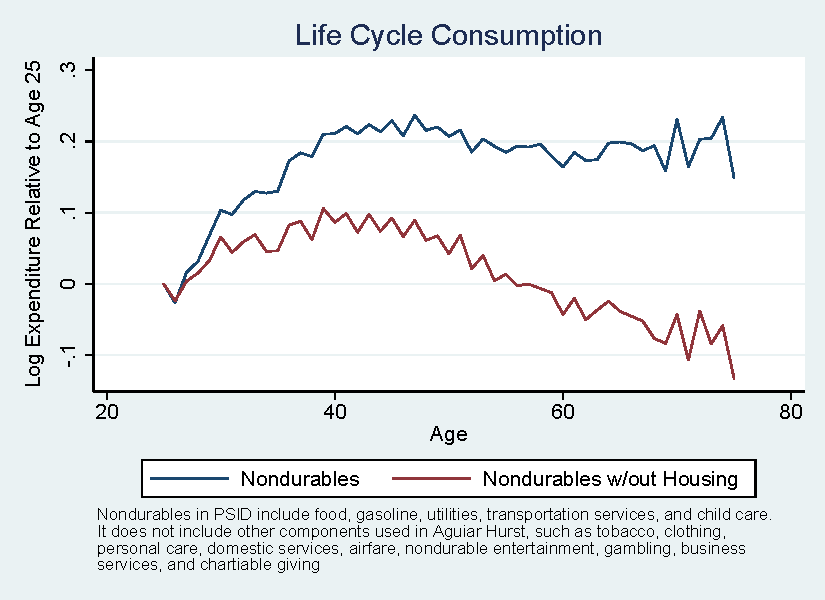
\includegraphics[width=0.9\textwidth]{../AguiarHurstReplication/Fig1.pdf}
\end{figure}

\pagebreak 
We replicate the method of Aguiar and Hurst (2013) to compute consumption dynamics over the life cycle. We use the Panel Study of Income Dynamics, whereas they use the CEX. These authors study the hump-shaped profile of nondurable expenditures and ask why nondurable expenditure declines during the second half of the life cycle, as seen in the red line of the first figure. The authors find that much of the decline is attributable to a decline in work related expenditures. This can be seen in the green line of the second figure.

\begin{figure}[h]
	%\caption{Life Cycle Consumption}
	\centering
	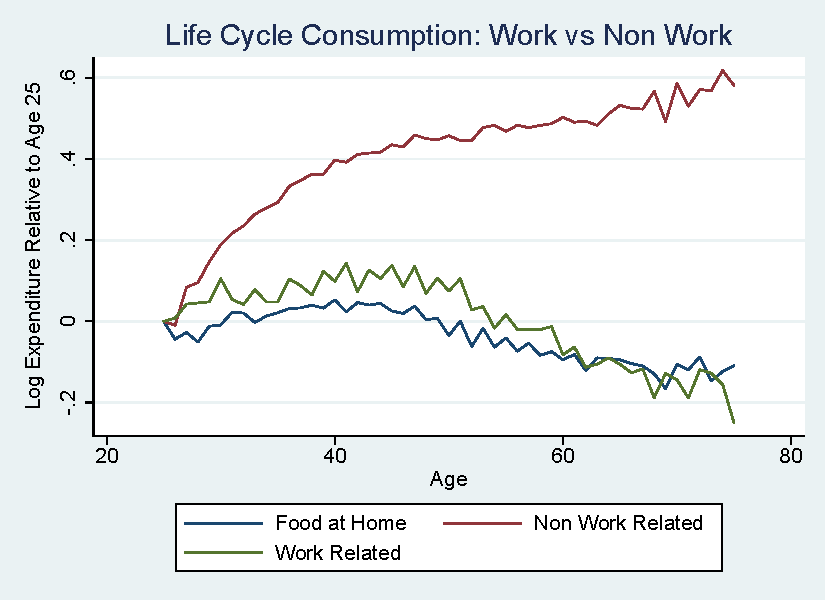
\includegraphics[width=0.7\textwidth]{../AguiarHurstReplication/Fig2.pdf}
\end{figure}

\begin{figure}[h]
	%\caption{Life Cycle Consumption}
	\centering
	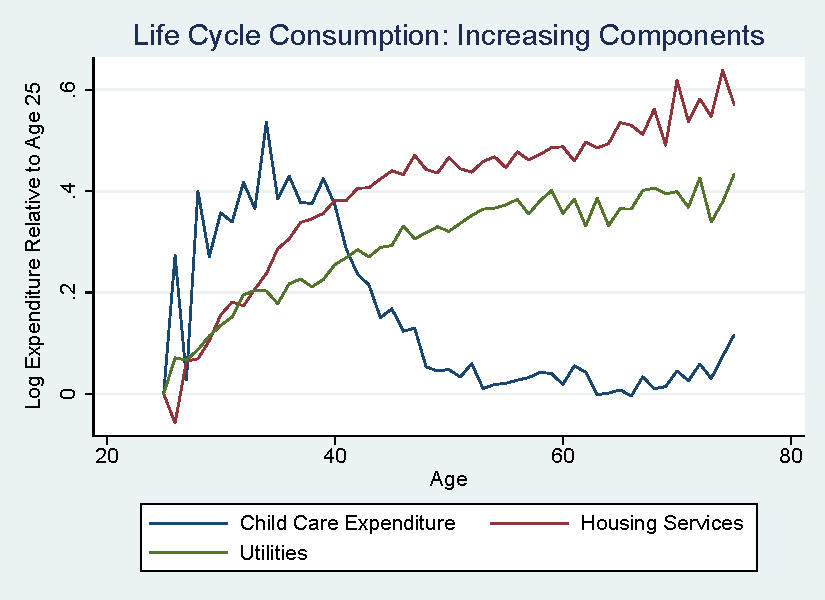
\includegraphics[width=0.7\textwidth]{../AguiarHurstReplication/Fig3a.pdf}
\end{figure}

\begin{figure}[h]
	%\caption{Life Cycle Consumption}
	\centering
	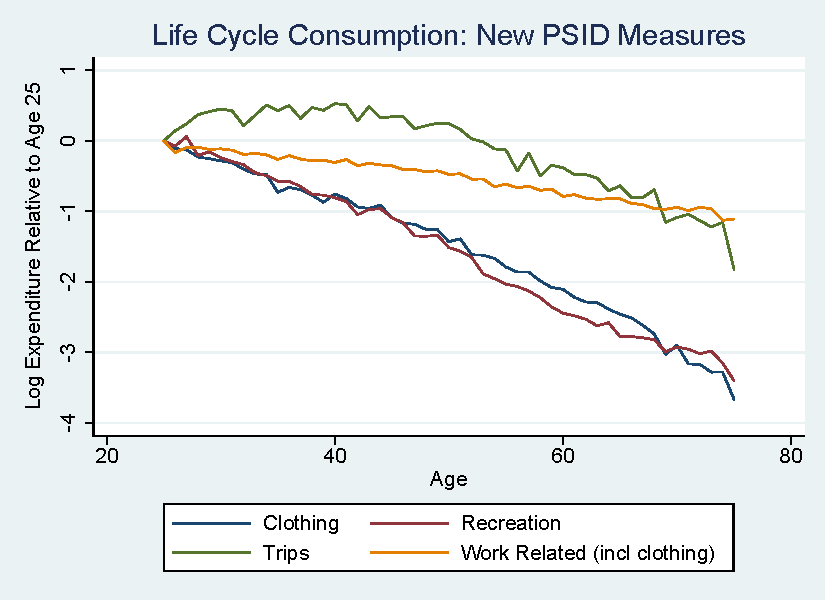
\includegraphics[width=0.9\textwidth]{../AguiarHurstReplication/Fig3c.pdf}
\end{figure}

\begin{figure}[h]
	%\caption{Life Cycle Consumption}
	\centering
	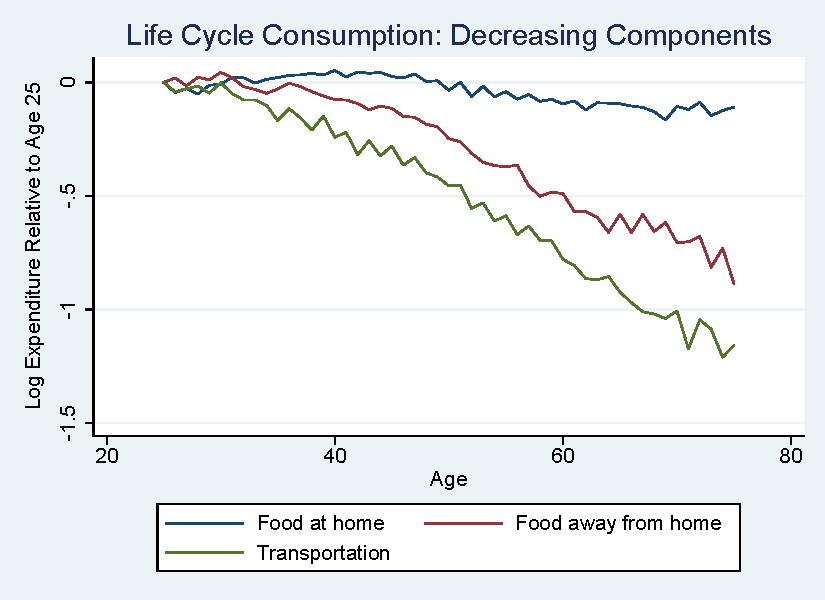
\includegraphics[width=0.9\textwidth]{../AguiarHurstReplication/Fig3b.pdf}
\end{figure}


\section{Life Cycle Consumption Dynamics (with HH FE)}

We extend the above analysis to take advantage of the longitudinal nature of the PSID. We add a household fixed effect to the age-period-cohort regression and take out the cohort effect. 

\begin{figure}[h]
	% \caption{Life Cycle Consumption}
	\centering
	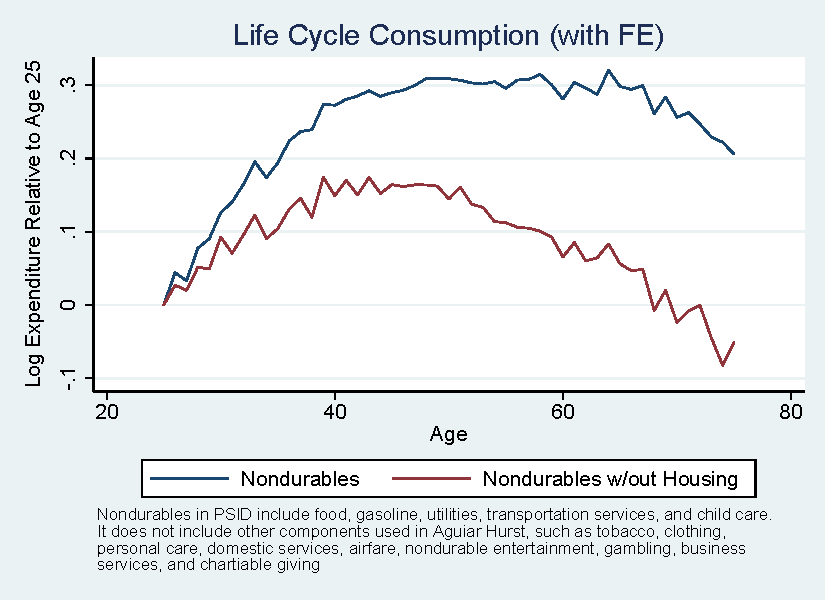
\includegraphics[width=0.9\textwidth]{../AguiarHurstReplication/Fig1_fe.pdf}
\end{figure}


\begin{figure}[h]
	%\caption{Life Cycle Consumption}
	\centering
	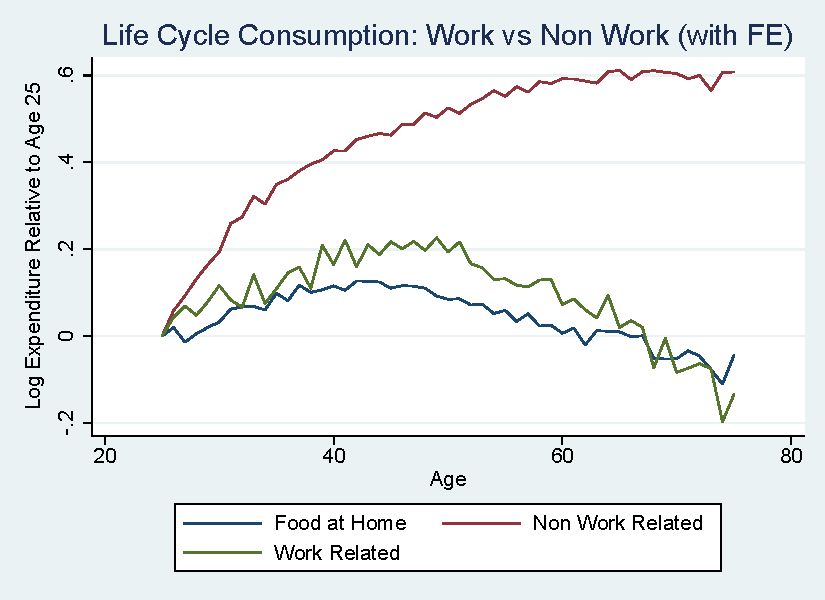
\includegraphics[width=0.9\textwidth]{../AguiarHurstReplication/Fig2_fe.pdf}
\end{figure}

\begin{figure}[h]
	%\caption{Life Cycle Consumption}
	\centering
	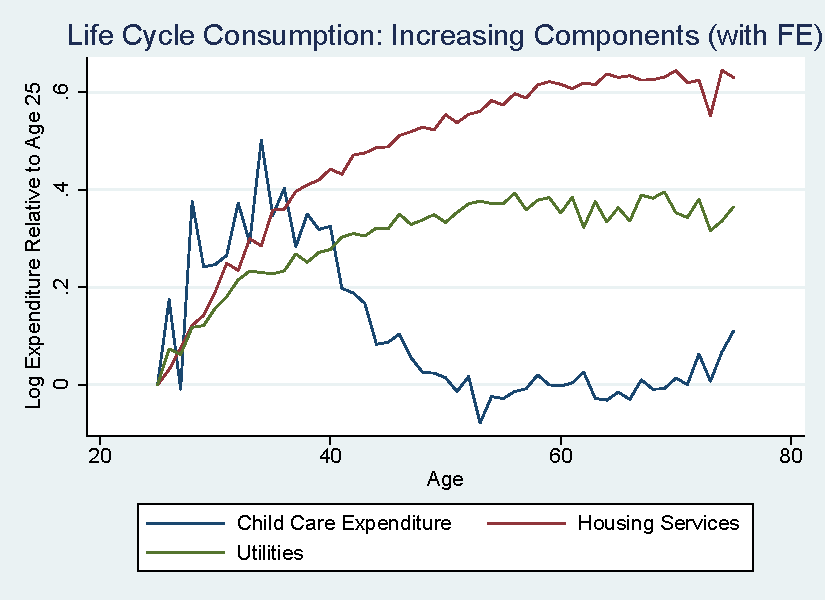
\includegraphics[width=0.9\textwidth]{../AguiarHurstReplication/Fig3a_fe.pdf}
\end{figure}

\begin{figure}[h]
	%\caption{Life Cycle Consumption}
	\centering
	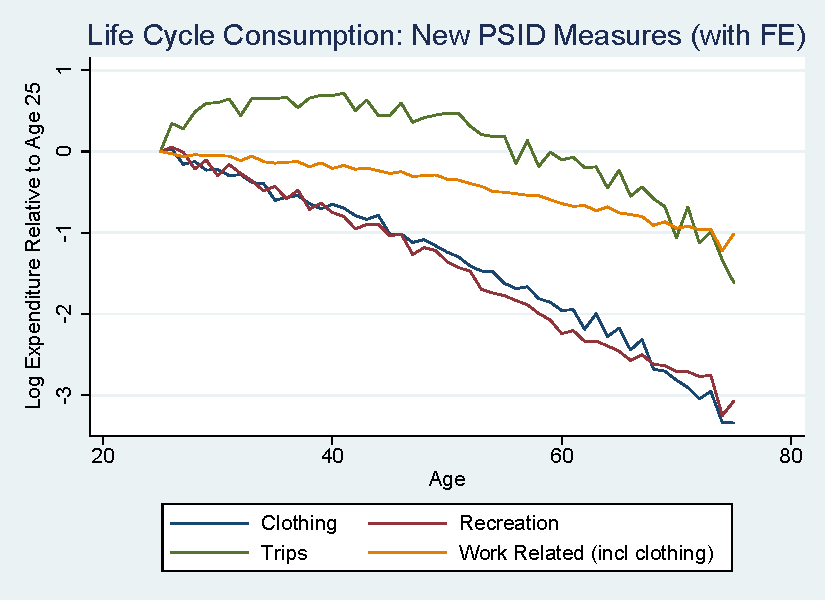
\includegraphics[width=0.9\textwidth]{../AguiarHurstReplication/Fig3c_fe.pdf}
\end{figure}

\begin{figure}[h]
	%\caption{Life Cycle Consumption}
	\centering
	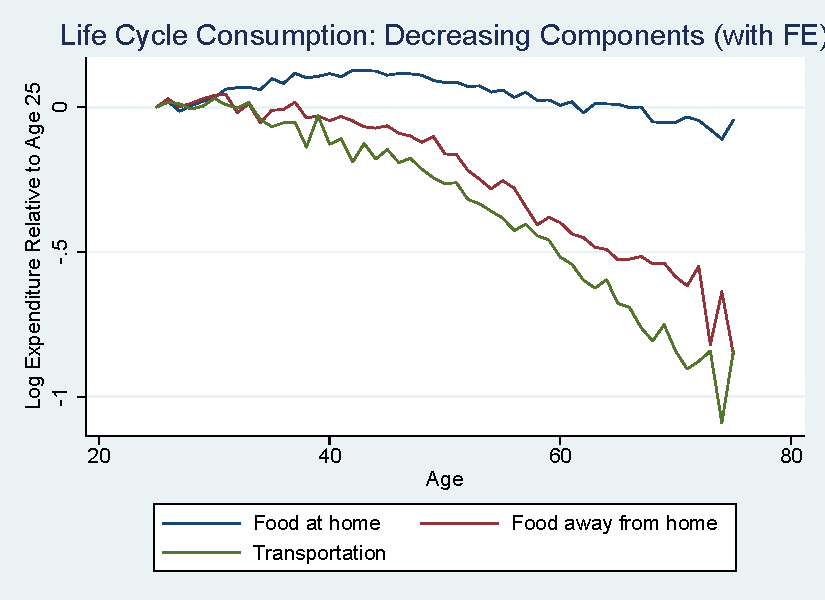
\includegraphics[width=0.9\textwidth]{../AguiarHurstReplication/Fig3b_fe.pdf}
\end{figure}


\section{Consumption around Retirement}

To explore the impact  of retirement, we compute mean consumption based on the retirement duration of the head of household (where the head retires at time zero). We explore the heterogeneous impact of retirement by quintiles based on social security income. 

While nondurable consumption (scaled for family size) declines for most of the population, we actually observe an increase in consumption for those in the top quintile. Similar behavior is apparent for the category of work related expenditure (in this case, gasoline/transportation/food away from home) where a decline is observed for the bottom four quintiles, but not the top quintile. Much of this can be attributed to food away from home, which declines for the bottom four quintiles, but not the top quintile. Finally, when we look at expenditure on trips/vacations, we observe a similarly large increase for households in the top quintile. 

\begin{figure}[h]
	%\caption{Life Cycle Consumption}
	\centering
	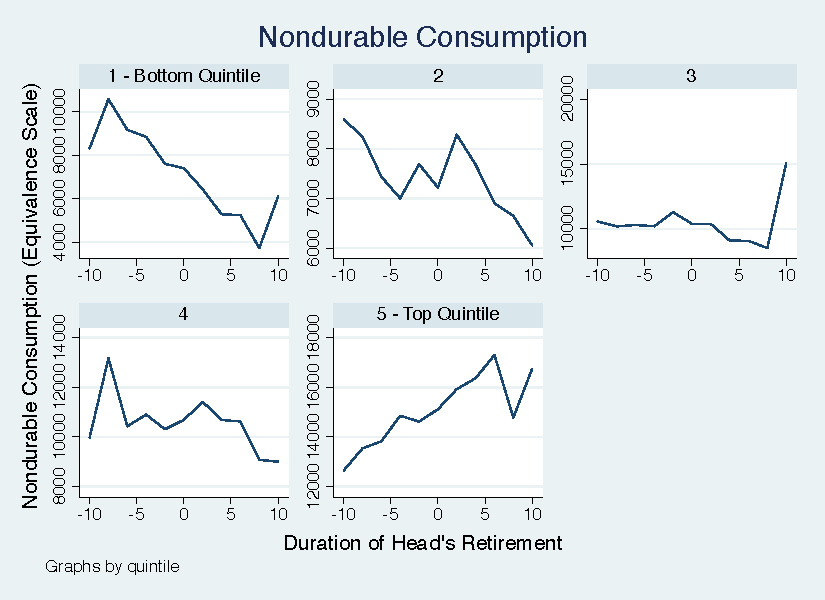
\includegraphics[width=1\textwidth]{../ConsumptionPostRetirement/expenditure_blundell_eq.pdf}
\end{figure}

\begin{figure}[h]
	%\caption{Life Cycle Consumption}
	\centering
	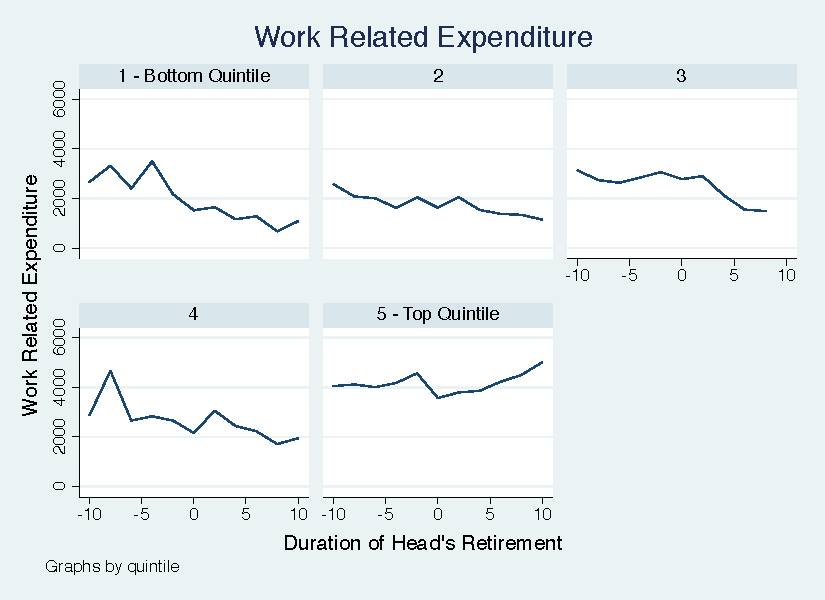
\includegraphics[width=0.9\textwidth]{../ConsumptionPostRetirement/work.pdf}
\end{figure}


\begin{figure}[h]
	%\caption{Life Cycle Consumption}
	\centering
	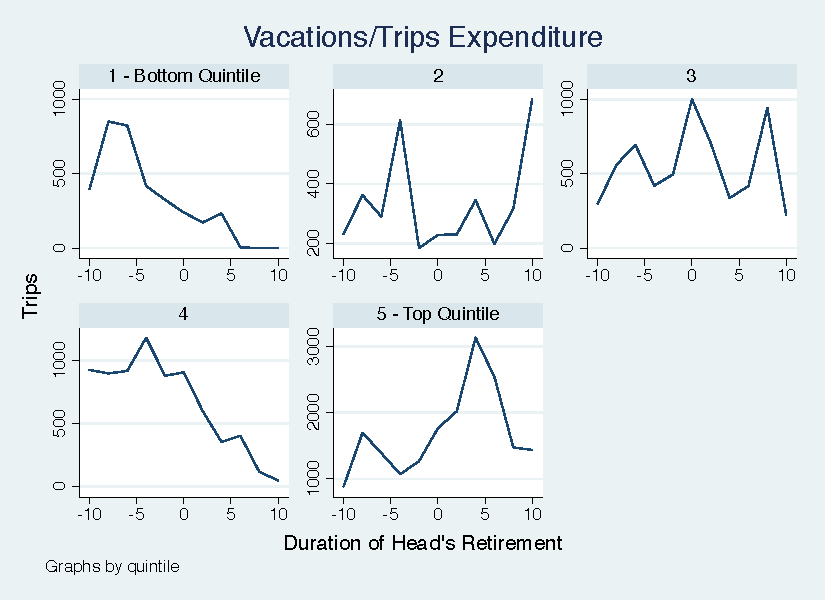
\includegraphics[width=0.9\textwidth]{../ConsumptionPostRetirement/trips.pdf}
\end{figure}

\begin{figure}[h]
	%\caption{Life Cycle Consumption}
	\centering
	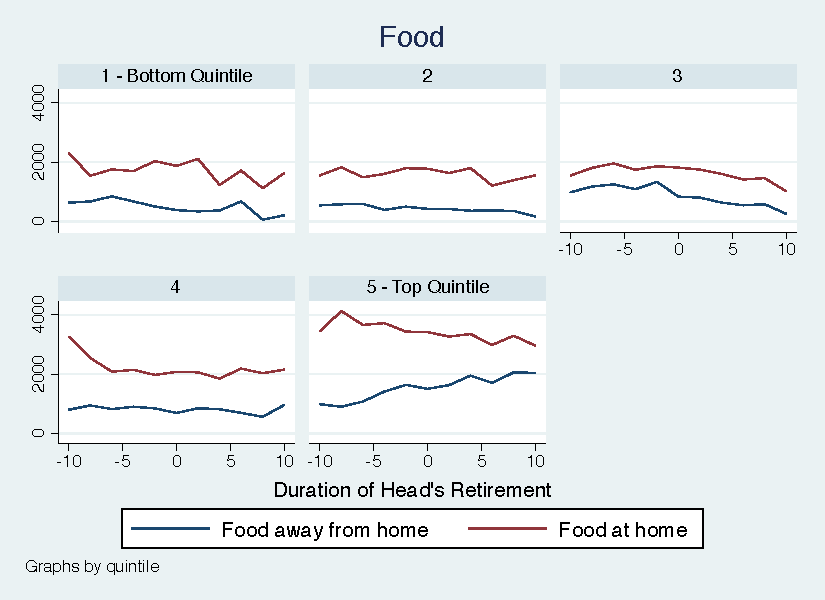
\includegraphics[width=0.9\textwidth]{../ConsumptionPostRetirement/food.pdf}
\end{figure}


Of course, these are just simple averages for now. The next step will be to integrate this analysis with the method of Aguiar and Hurst. Then we can look at the impact of retirement on consumption while controlling for age, period, cohort, marital status, and family size effects. This will hopefully allow us to get a better picture of the heterogeneous impact of retirement.

\section{Consumption around Retirement by Tertile Pre-2005}

To further explore the impact  of retirement, we compute the mean consumption based on tertile for different nondurable categories. 

\begin{figure}[h]
	%\caption{Life Cycle Consumption}
	\centering
	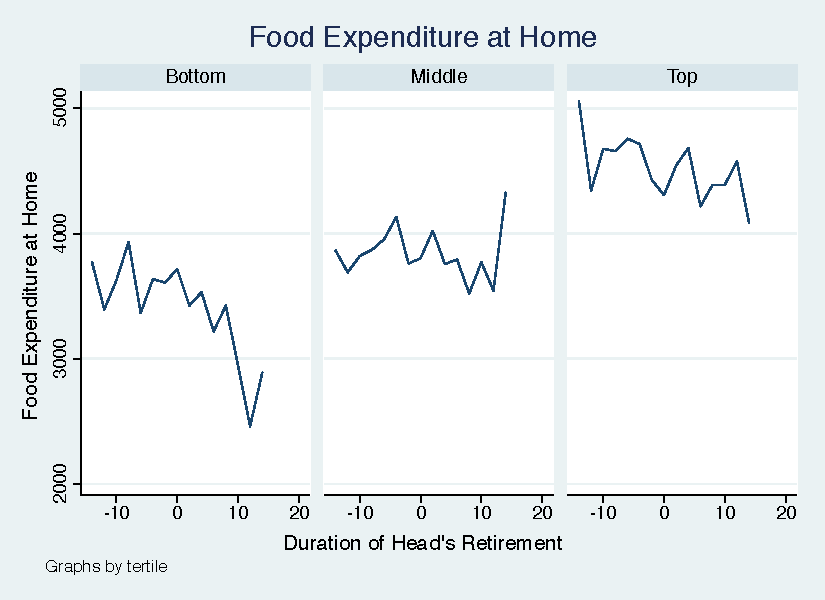
\includegraphics[width=0.9\textwidth]{../ConsumptionPostRetirement/Tertile_1/total_foodexp_home_real.pdf}
\end{figure}

\clearpage

\section{Imputed Expenditure versus Sum of Categorical}

\begin{figure}[h]
	\caption{For categories before 2005}
	\centering
	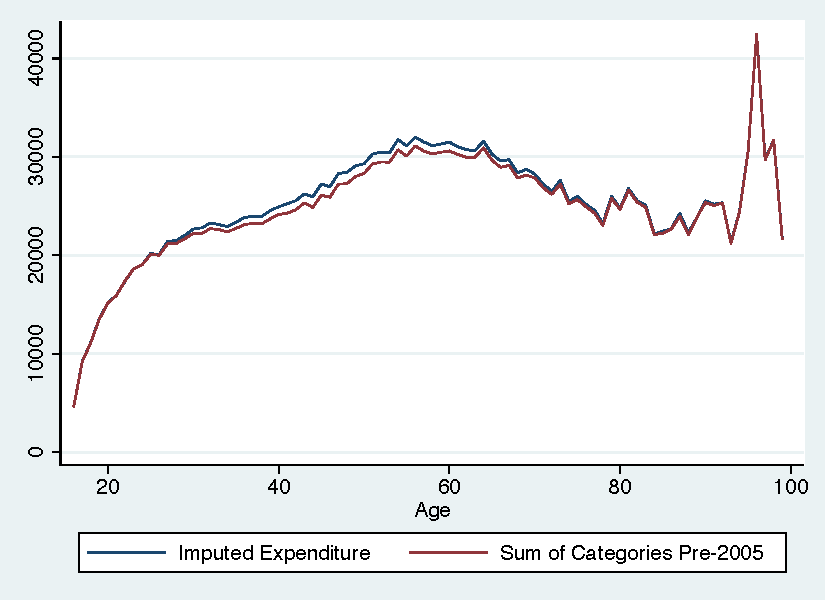
\includegraphics[width=0.8\textwidth]{../ConsumptionPostRetirement/Comparision_of_imputed_and_categorical_age.pdf}
\end{figure}

\begin{figure}[h]
	\caption{For categories before 2005}
	\centering
	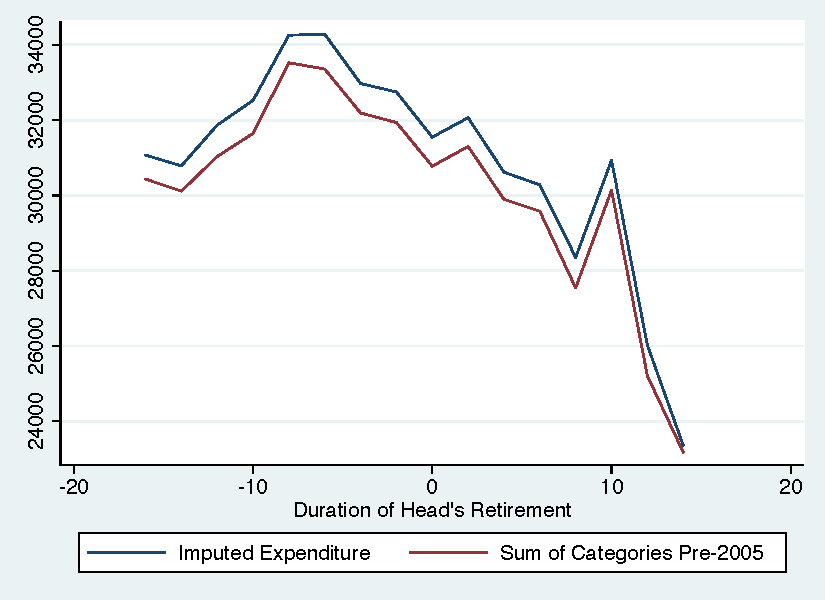
\includegraphics[width=0.8\textwidth]{../ConsumptionPostRetirement/Comparision_of_imputed_and_categorical_ret.pdf}
\end{figure}


\section{Imputed Expenditure versus Sum of Categorical}

\begin{figure}[h]
	\caption{For categories before 2005}
	\centering
	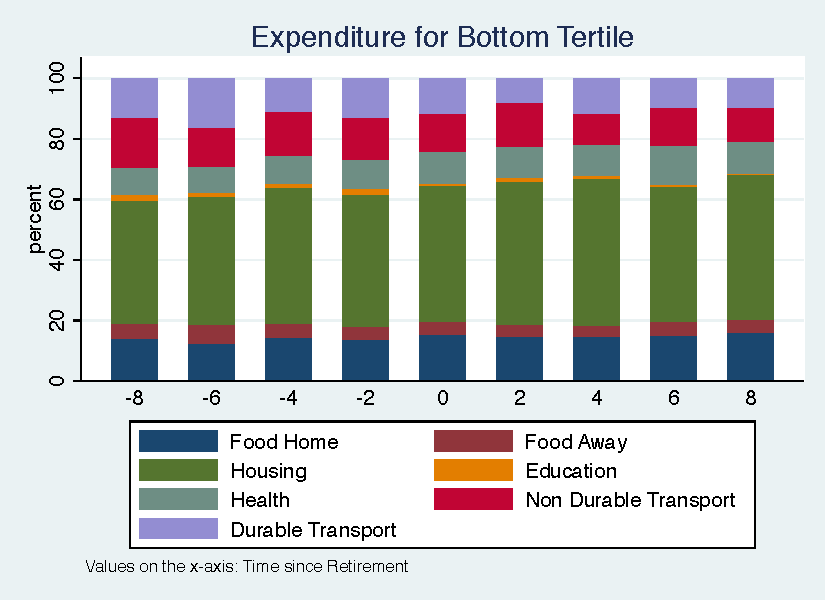
\includegraphics[width=0.8\textwidth]{../ConsumptionPostRetirement/Tertile_Bar/tertile1.pdf}
\end{figure}

\begin{figure}[h]
	\caption{For categories before 2005}
	\centering
	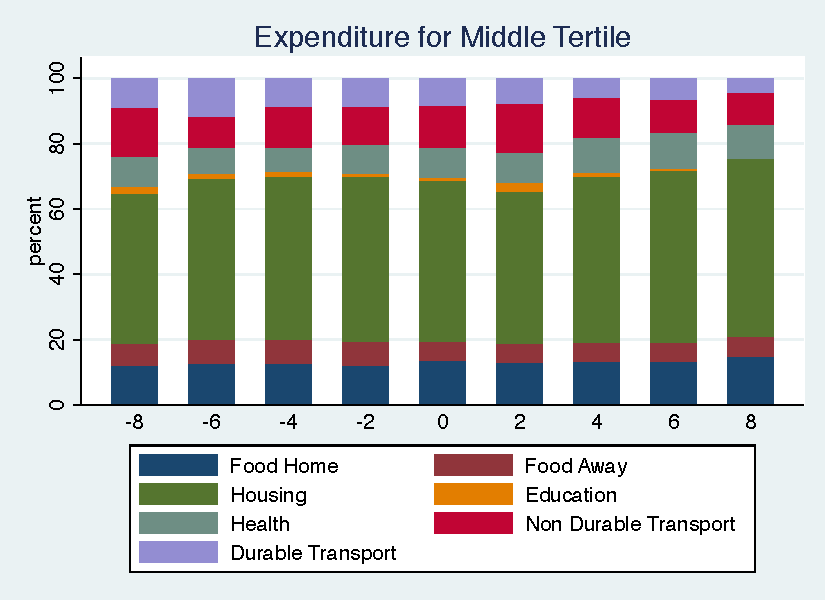
\includegraphics[width=0.8\textwidth]{../ConsumptionPostRetirement/Tertile_Bar/tertile2.pdf}
\end{figure}

\begin{figure}[h]
	\caption{For categories before 2005}
	\centering
	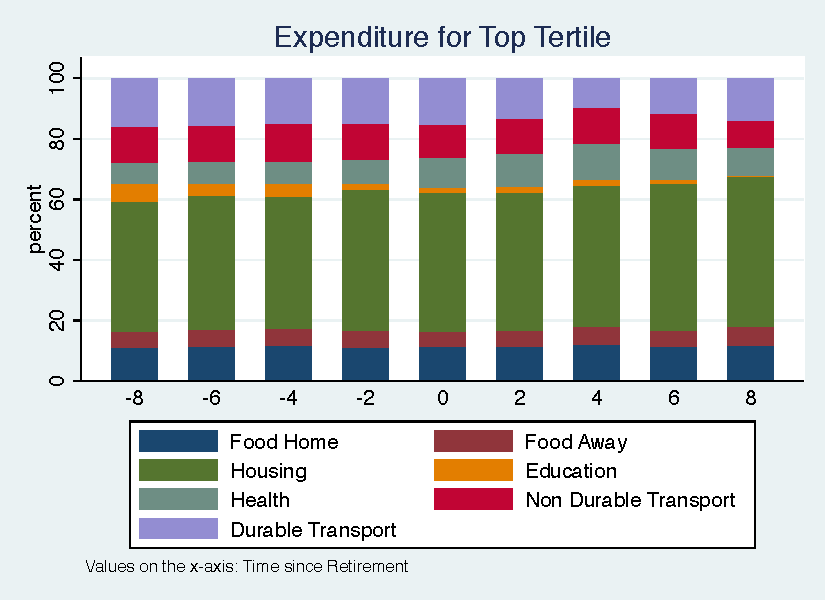
\includegraphics[width=0.8\textwidth]{../ConsumptionPostRetirement/Tertile_Bar/tertile3.pdf}
\end{figure}



\section{Bar Graphs for Categorical Expenditure}

\begin{figure}[h]
	\caption{1 - Spouse never works}
	\centering
	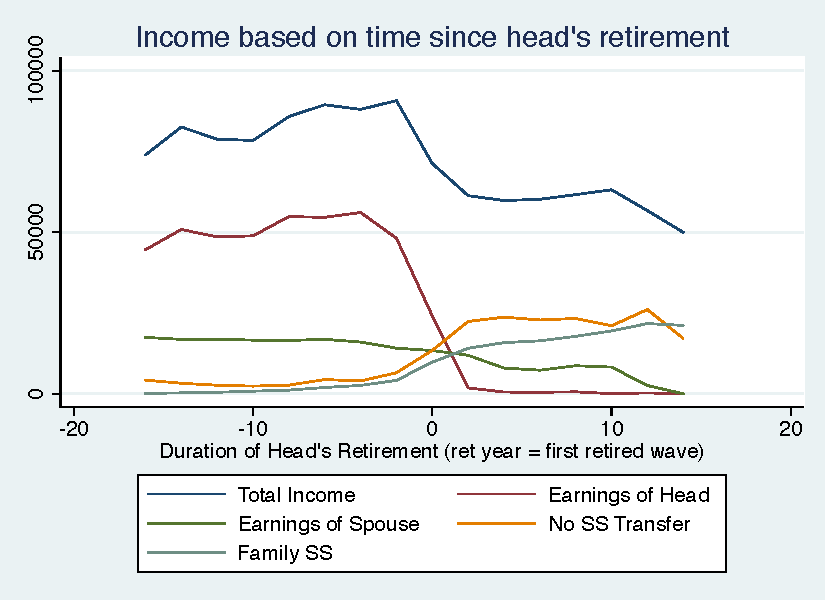
\includegraphics[width=0.8\textwidth]{../IncomeAroundRetirement/Income_with_spouse_definition_1.pdf}
\end{figure}

\begin{figure}[h]
	\caption{2 - Spouse always works}
	\centering
	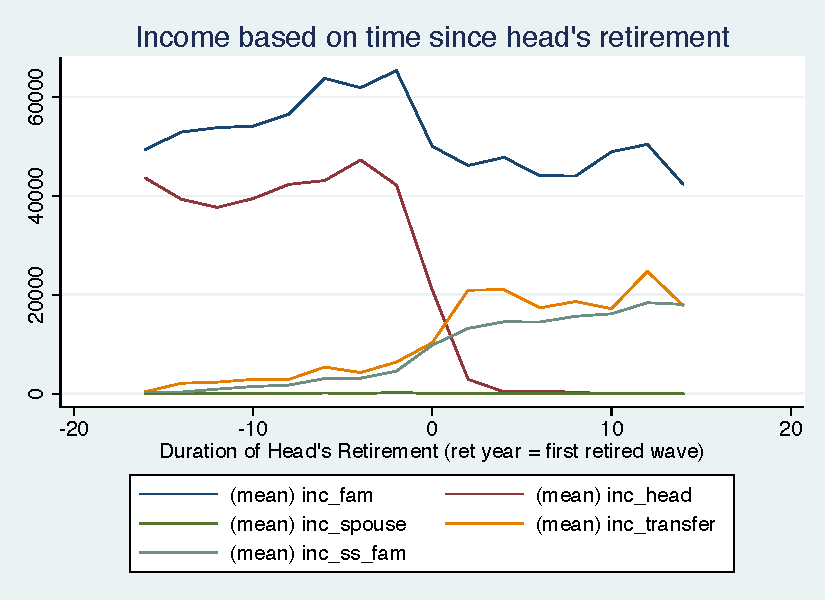
\includegraphics[width=0.8\textwidth]{../IncomeAroundRetirement/Income_with_spouse_definition_2.pdf}
\end{figure}

\begin{figure}[h]
	\caption{3 - Spouse has same retirement transition +/- wave}
	\centering
	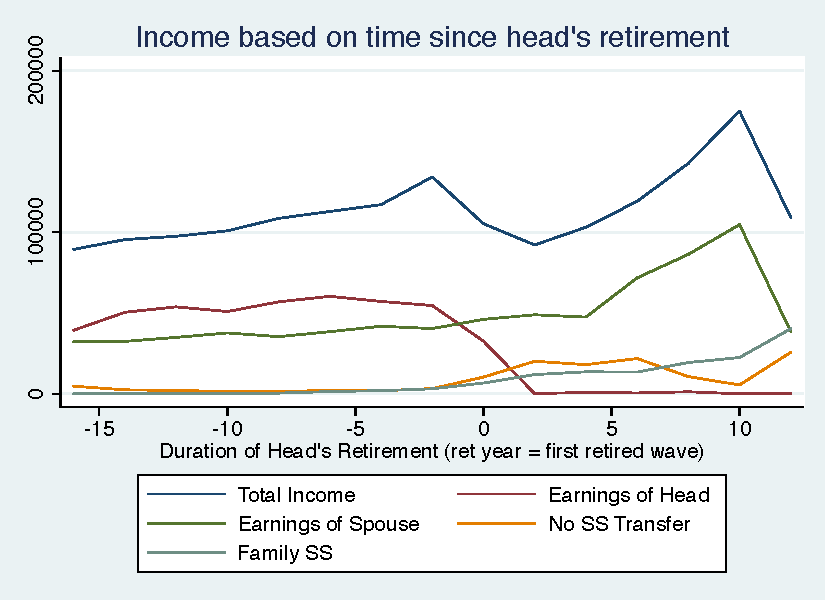
\includegraphics[width=0.8\textwidth]{../IncomeAroundRetirement/Income_with_spouse_definition_3.pdf}
\end{figure}

\begin{figure}[h]
	\caption{4 - Spouse has a different retirement transition}
	\centering
	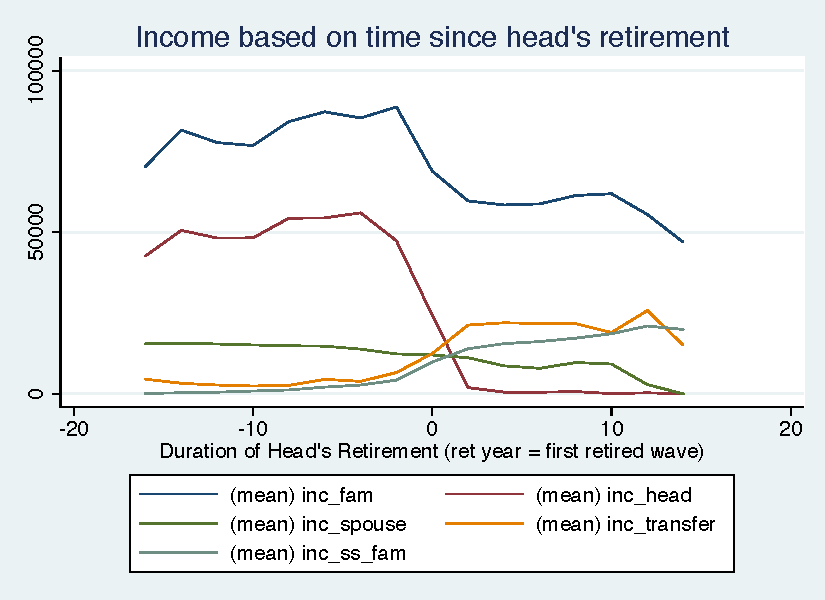
\includegraphics[width=0.8\textwidth]{../IncomeAroundRetirement/Income_with_spouse_definition_4.pdf}
\end{figure}

\begin{figure}[h]
	\caption{5 - Ignoring the spouse}
	\centering
	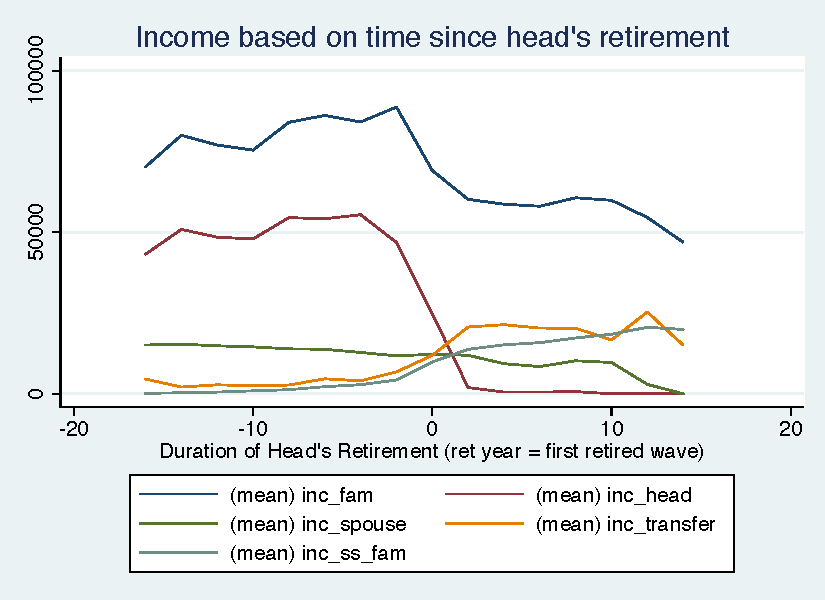
\includegraphics[width=0.8\textwidth]{../IncomeAroundRetirement/Income_with_spouse_definition_5.pdf}
\end{figure}


\clearpage
\section{Expenditure based on tertiles for spouse retirement}

\subsection{Spouse Never Works}

\begin{figure}[h]
	\caption{1 - Spouse never works(Smoothed)}
	\centering
	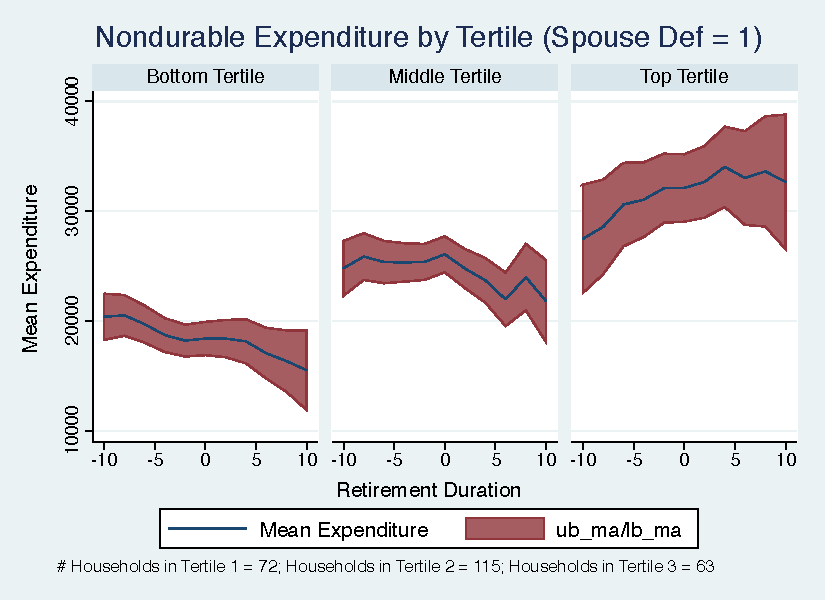
\includegraphics[width=0.6\textwidth]{../ConsumptionPostRetirement_by_SpouseDef/Smoothed/spouse_def_1.pdf}
\end{figure}

\begin{figure}[h]
	\caption{1 - Spouse never works(Unsmoothed)}
	\centering
	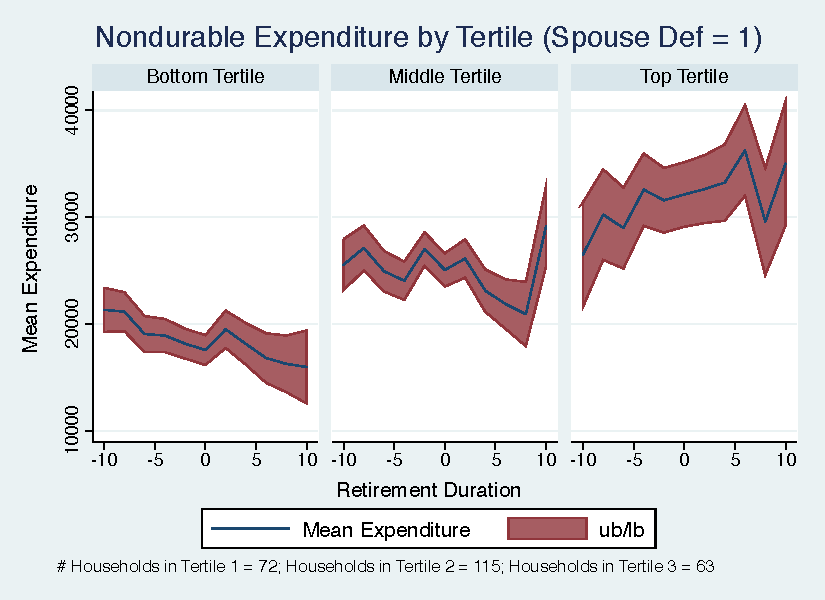
\includegraphics[width=0.6\textwidth]{../ConsumptionPostRetirement_by_SpouseDef/UnSmoothed/spouse_def_1.pdf}
\end{figure}
\clearpage


\subsection{Spouse always works}
\begin{figure}[h]
	\caption{2 - Spouse always works(Smoothed)}
	\centering
	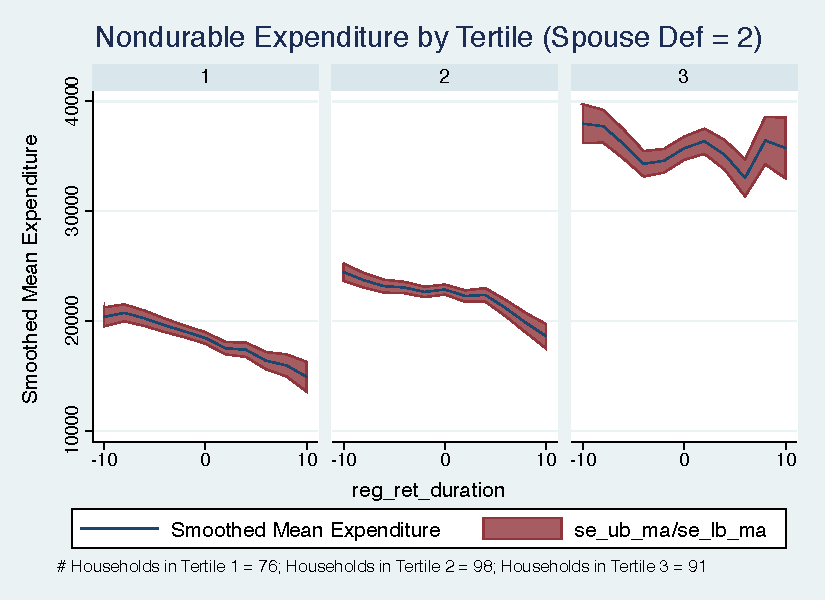
\includegraphics[width=0.6\textwidth]{../ConsumptionPostRetirement_by_SpouseDef/Smoothed/spouse_def_2.pdf}
\end{figure}

\begin{figure}[h]
	\caption{2 - Spouse always works(Unsmoothed)}
	\centering
	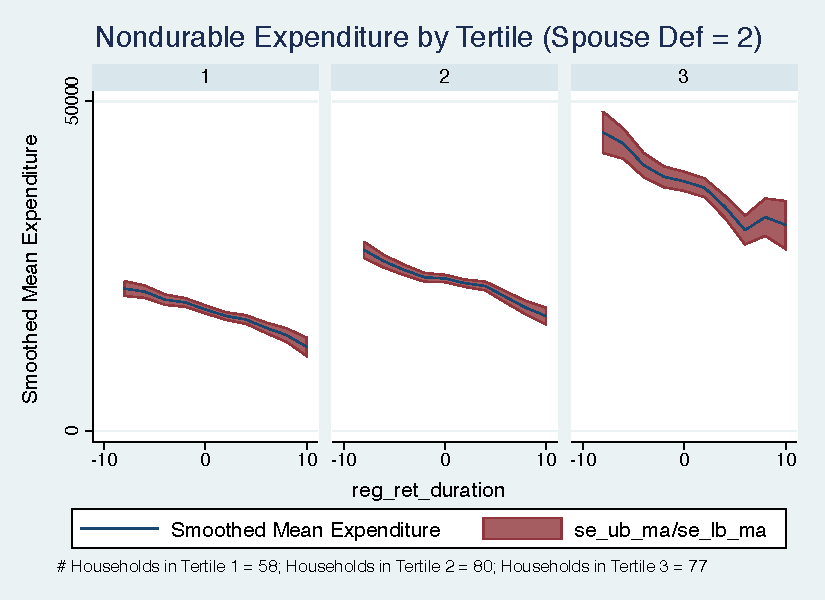
\includegraphics[width=0.6\textwidth]{../ConsumptionPostRetirement_by_SpouseDef/UNSmoothed/spouse_def_2.pdf}
\end{figure}
\clearpage

\subsection{Same retirement transition +/- wave}
\begin{figure}[h]
	\caption{3 - Spouse has same retirement transition +/- wave (Smoothed)}
	\centering
	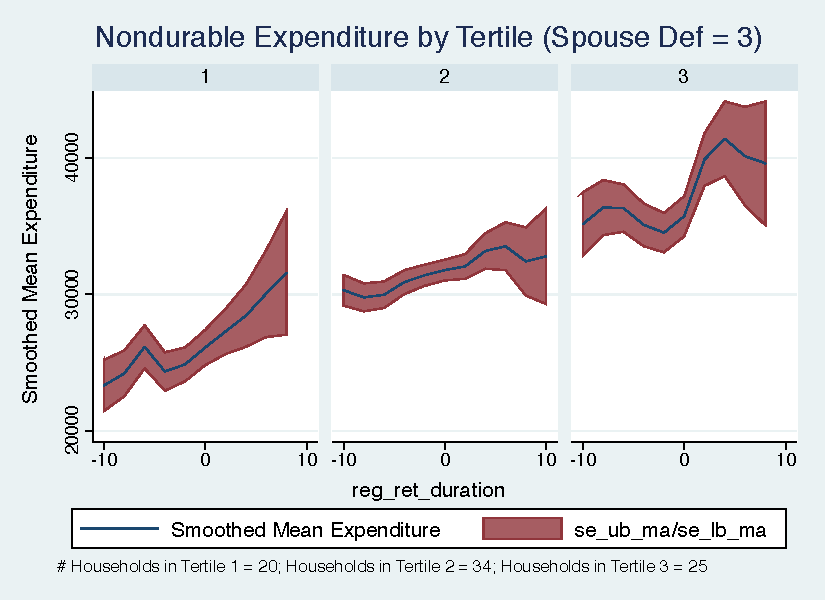
\includegraphics[width=0.6\textwidth]{../ConsumptionPostRetirement_by_SpouseDef/Smoothed/spouse_def_3.pdf}
\end{figure}

\begin{figure}[h]
	\caption{3 - Spouse has same retirement transition +/- wave(Unsmoothed)}
	\centering
	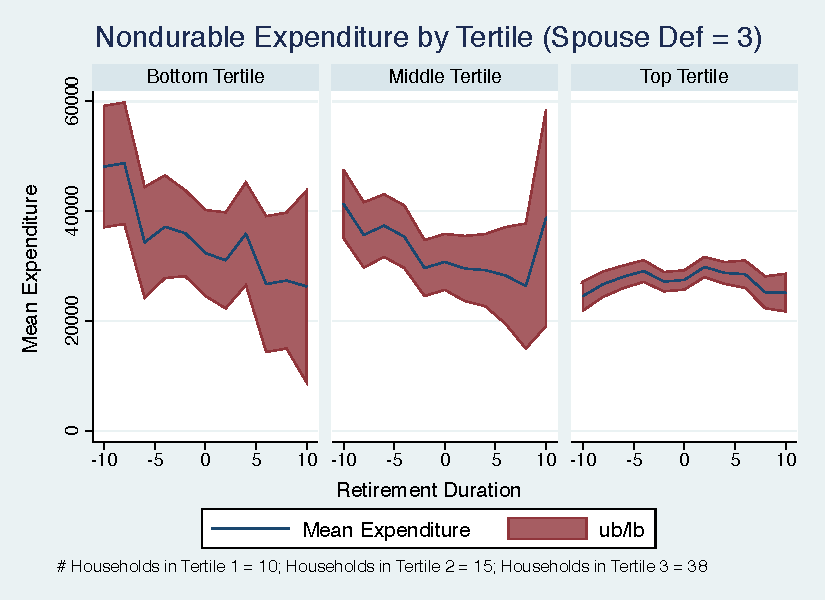
\includegraphics[width=0.6\textwidth]{../ConsumptionPostRetirement_by_SpouseDef/UnSmoothed/spouse_def_3.pdf}
\end{figure}
\clearpage


\subsection{Different retirement transition}
\begin{figure}[h]
	\caption{4 - Spouse has a different retirement transition(Smoothed)}
	\centering
	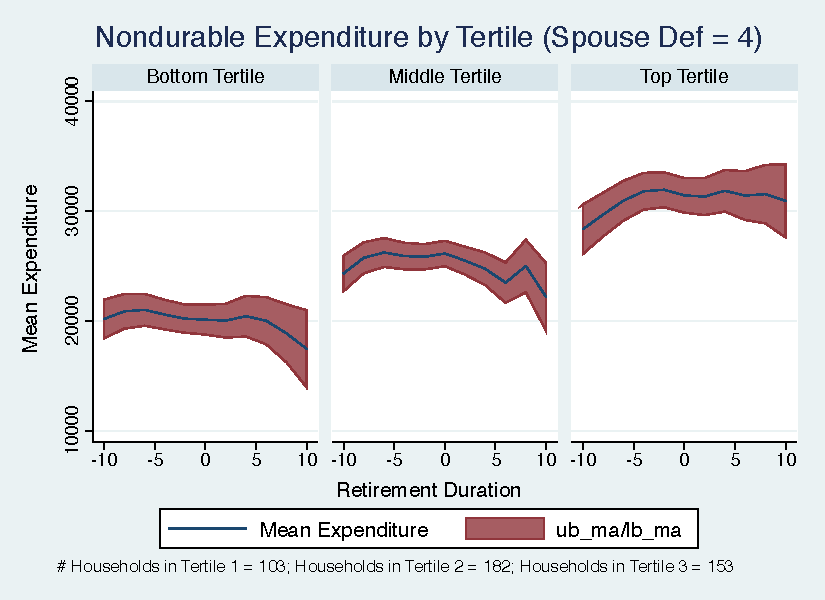
\includegraphics[width=0.6\textwidth]{../ConsumptionPostRetirement_by_SpouseDef/Smoothed/spouse_def_4.pdf}
\end{figure}

\begin{figure}[h]
	\caption{4 - Spouse has a different retirement transition(Unsmoothed)}
	\centering
	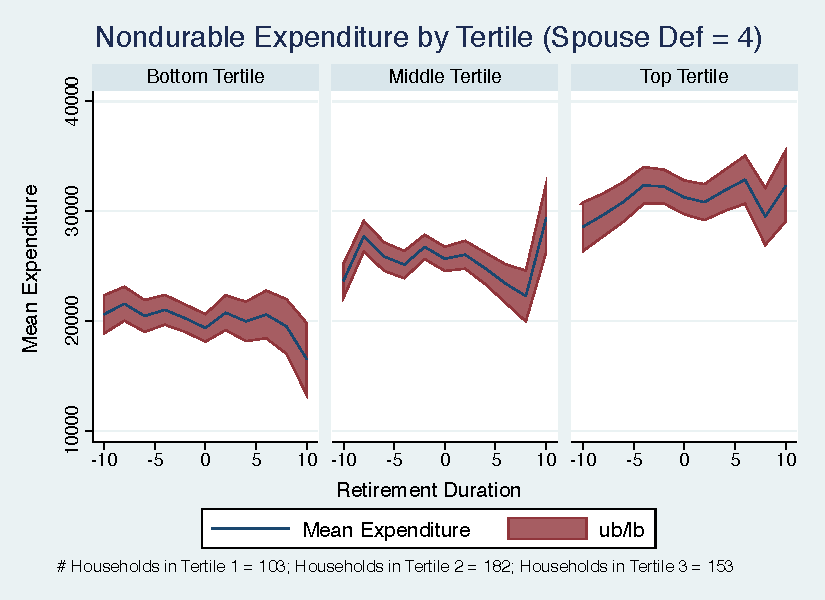
\includegraphics[width=0.6\textwidth]{../ConsumptionPostRetirement_by_SpouseDef/UnSmoothed/spouse_def_4.pdf}
\end{figure}
\clearpage


\subsection{Ignoring the spouse}

\begin{figure}[h]
	\caption{5 - Ignoring the spouse (Smoothed)}
	\centering
	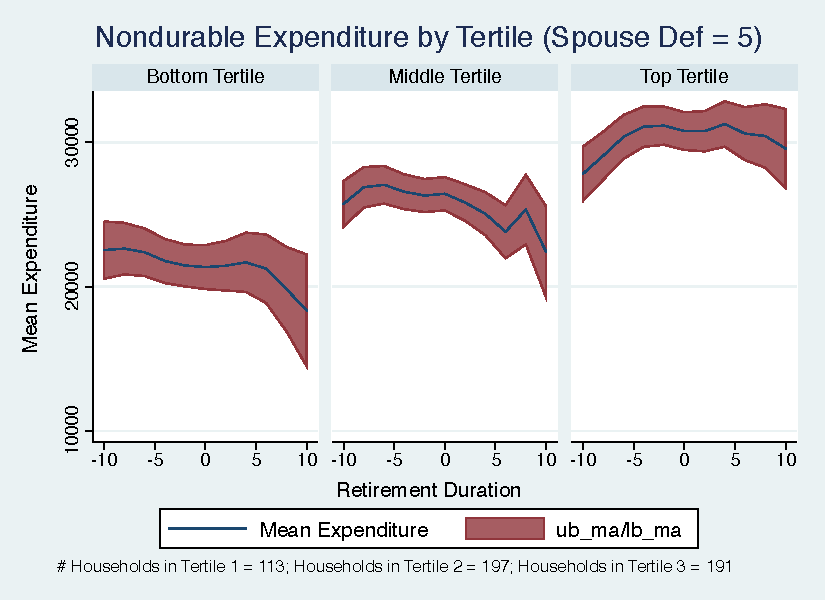
\includegraphics[width=0.6\textwidth]{../ConsumptionPostRetirement_by_SpouseDef/Smoothed/spouse_def_5.pdf}
\end{figure}

\begin{figure}[h]
	\caption{5 - Ignoring the spouse(Unsmoothed)}
	\centering
	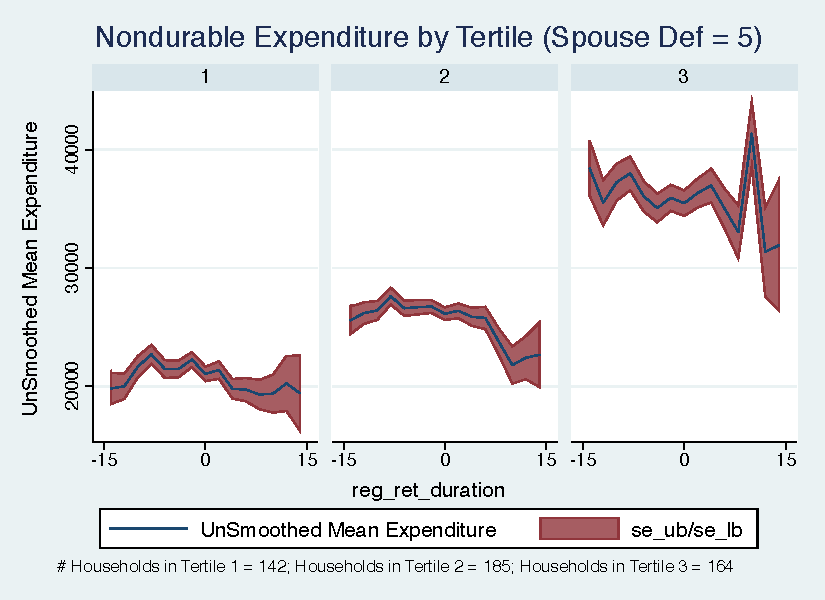
\includegraphics[width=0.6\textwidth]{../ConsumptionPostRetirement_by_SpouseDef/UnSmoothed/spouse_def_5.pdf}
\end{figure}

\clearpage

\section{Categorical Expenditure Based on Spouse Defination}

\subsection{1- Spouse Never Works}

\begin{figure}[h]
	\caption{Food Expenditure at Home}
	\centering
	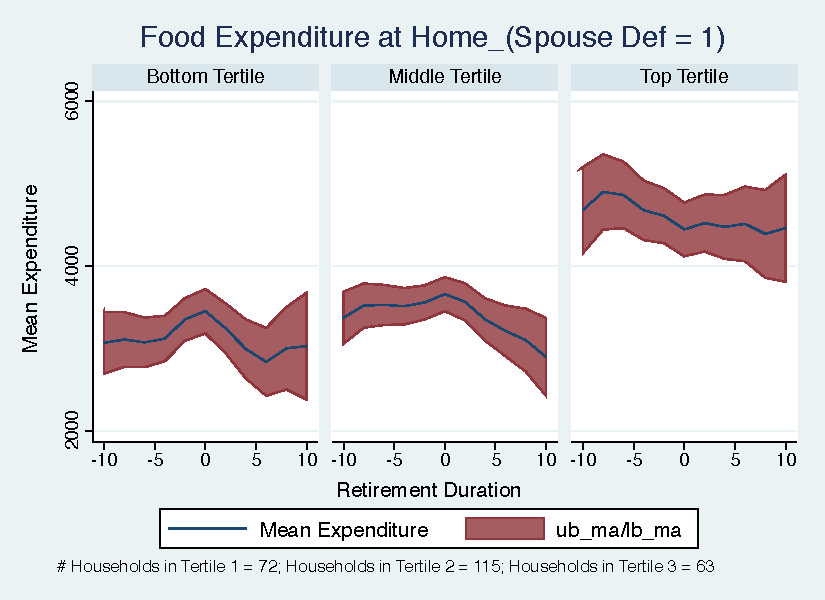
\includegraphics[width=0.6\textwidth]{../ConsumptionPostRetirement_by_SpouseDef_Cats/Smoothed/1/spouse_def_total_foodexp_home_real.pdf}
\end{figure}


\begin{figure}[h]
	\caption{Food Expenditure Away from Home}
	\centering
	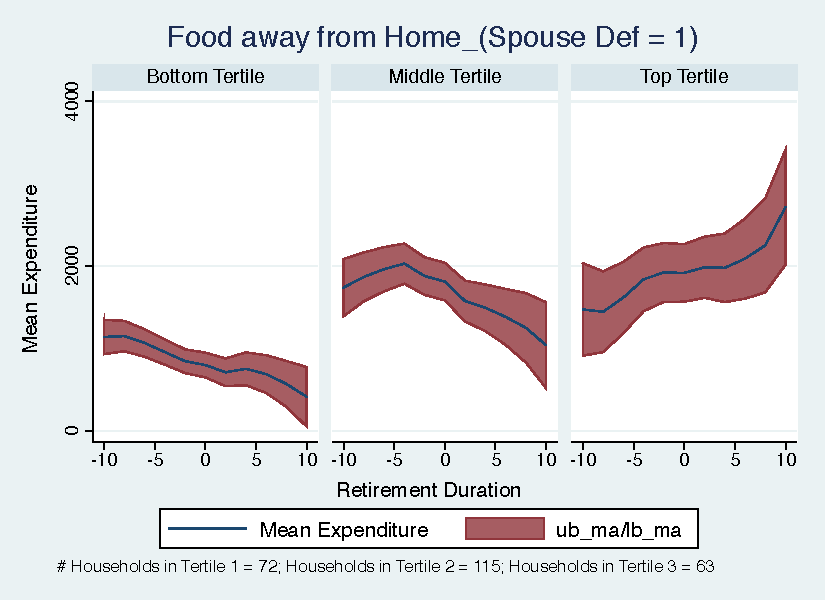
\includegraphics[width=0.6\textwidth]{../ConsumptionPostRetirement_by_SpouseDef_Cats/Smoothed/1/spouse_def_total_foodexp_away_real.pdf}
\end{figure}

\clearpage

\begin{figure}[h]
	\caption{Expenditure on Housing}
	\centering
	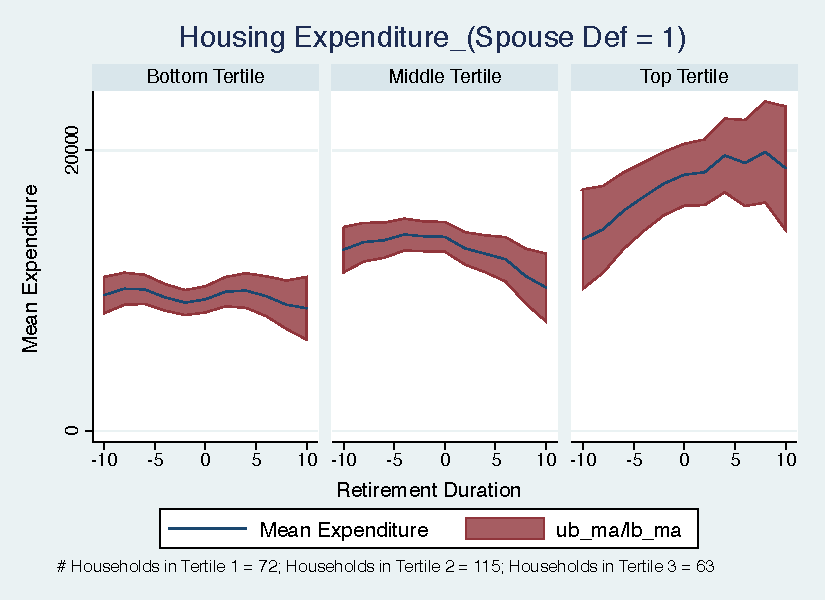
\includegraphics[width=0.6\textwidth]{../ConsumptionPostRetirement_by_SpouseDef_Cats/Smoothed/1/spouse_def_total_housing_real.pdf}
\end{figure}


\begin{figure}[h]
	\caption{Expenditure on Education}
	\centering
	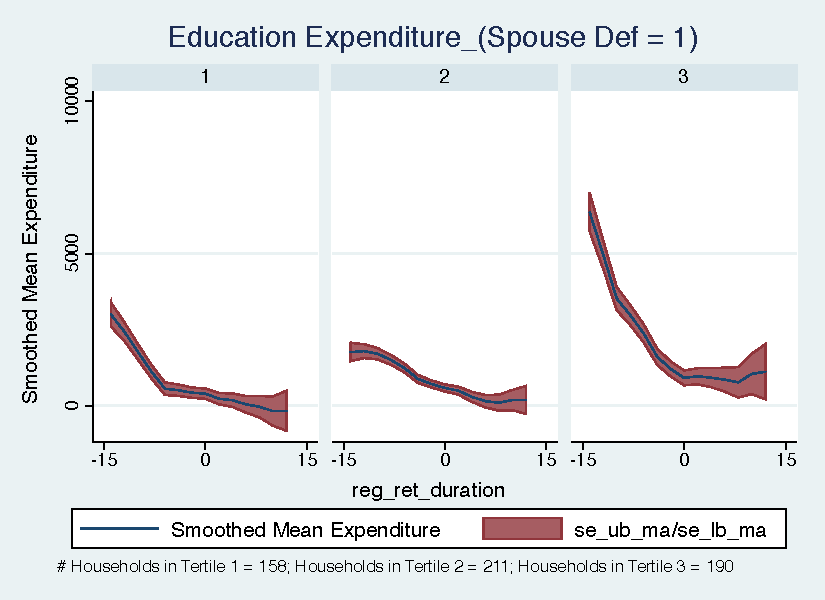
\includegraphics[width=0.6\textwidth]{../ConsumptionPostRetirement_by_SpouseDef_Cats/Smoothed/1/spouse_def_total_education_real.pdf}
\end{figure}
\clearpage

\begin{figure}[h]
	\caption{Expenditure on Health}
	\centering
	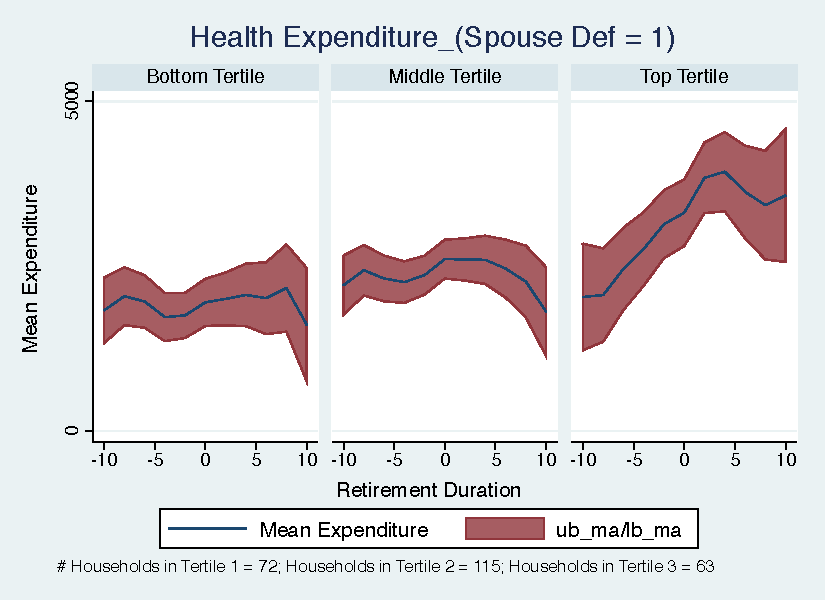
\includegraphics[width=0.6\textwidth]{../ConsumptionPostRetirement_by_SpouseDef_Cats/Smoothed/1/spouse_def_total_healthexpense_real.pdf}
\end{figure}


\begin{figure}[h]
	\caption{Expenditure on Non-Durable Transport}
	\centering
	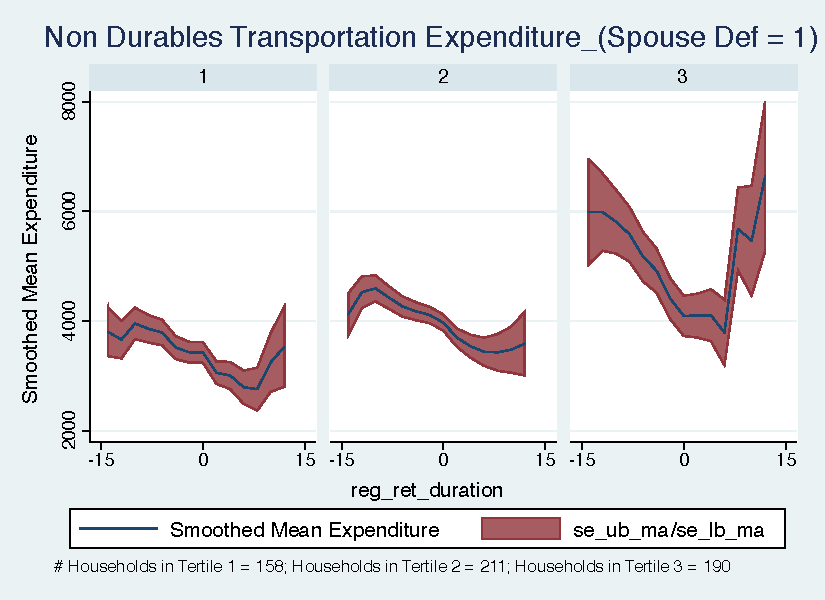
\includegraphics[width=0.6\textwidth]{../ConsumptionPostRetirement_by_SpouseDef_Cats/Smoothed/1/spouse_def_total_transport_real.pdf}
\end{figure}
\clearpage

\subsection{2- Spouse Always Works}

\begin{figure}[h]
	\caption{Food Expenditure at Home}
	\centering
	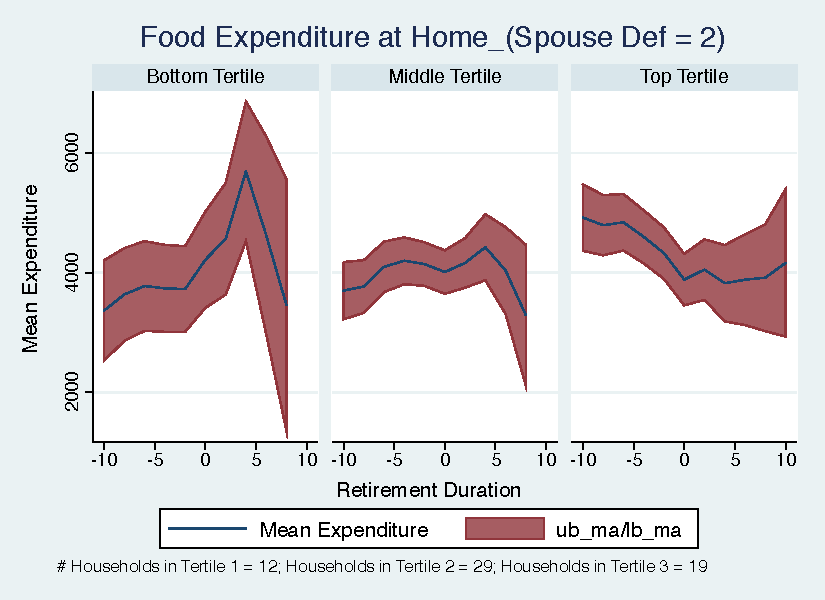
\includegraphics[width=0.6\textwidth]{../ConsumptionPostRetirement_by_SpouseDef_Cats/Smoothed/2/spouse_def_total_foodexp_home_real.pdf}
\end{figure}


\begin{figure}[h]
	\caption{Food Expenditure Away from Home}
	\centering
	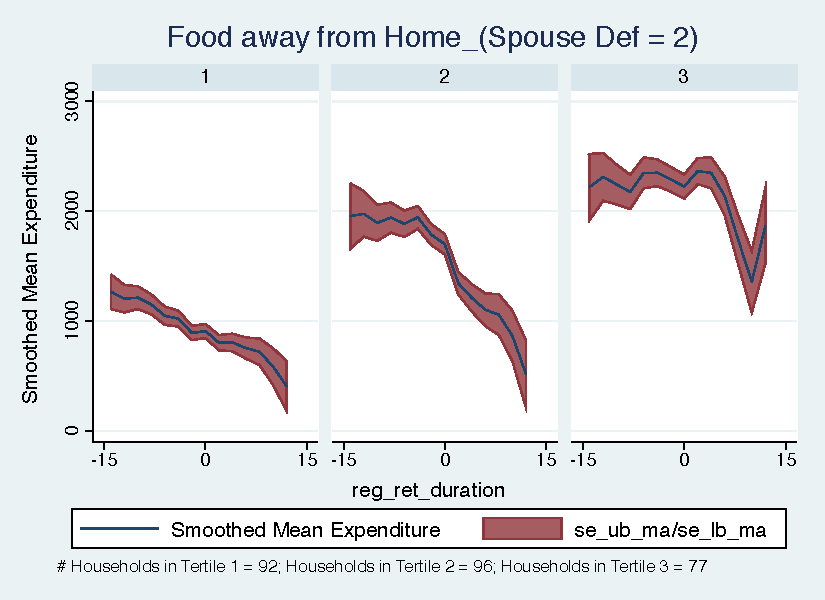
\includegraphics[width=0.6\textwidth]{../ConsumptionPostRetirement_by_SpouseDef_Cats/Smoothed/2/spouse_def_total_foodexp_away_real.pdf}
\end{figure}

\clearpage

\begin{figure}[h]
	\caption{Expenditure on Housing}
	\centering
	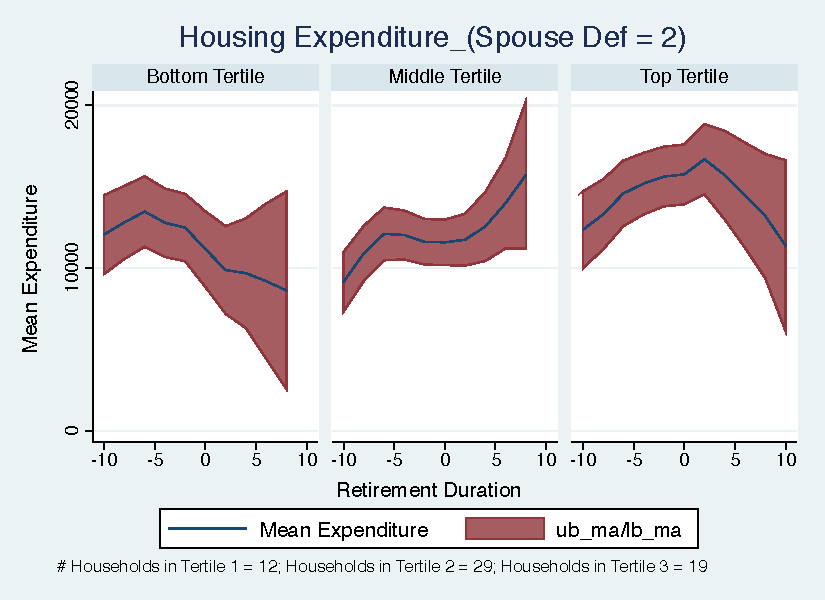
\includegraphics[width=0.6\textwidth]{../ConsumptionPostRetirement_by_SpouseDef_Cats/Smoothed/2/spouse_def_total_housing_real.pdf}
\end{figure}


\begin{figure}[h]
	\caption{Expenditure on Education}
	\centering
	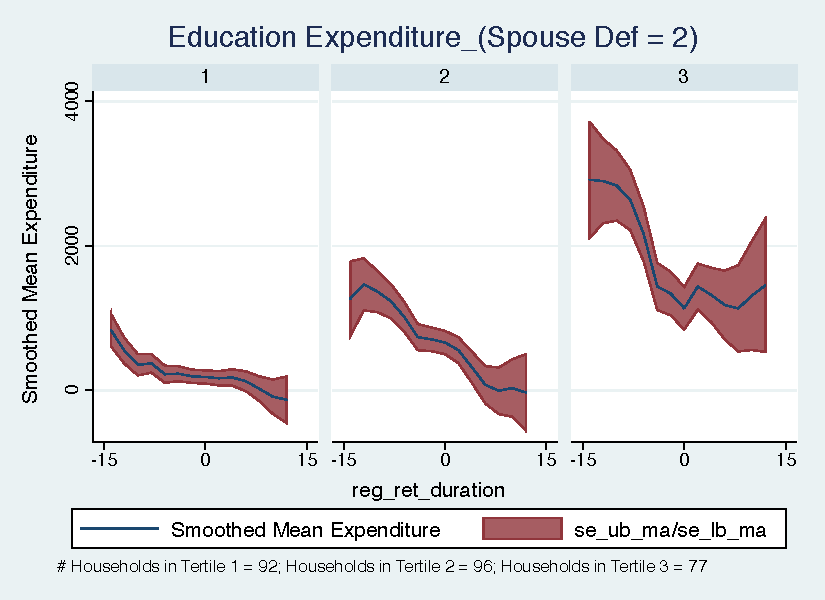
\includegraphics[width=0.6\textwidth]{../ConsumptionPostRetirement_by_SpouseDef_Cats/Smoothed/2/spouse_def_total_education_real.pdf}
\end{figure}
\clearpage

\begin{figure}[h]
	\caption{Expenditure on Health}
	\centering
	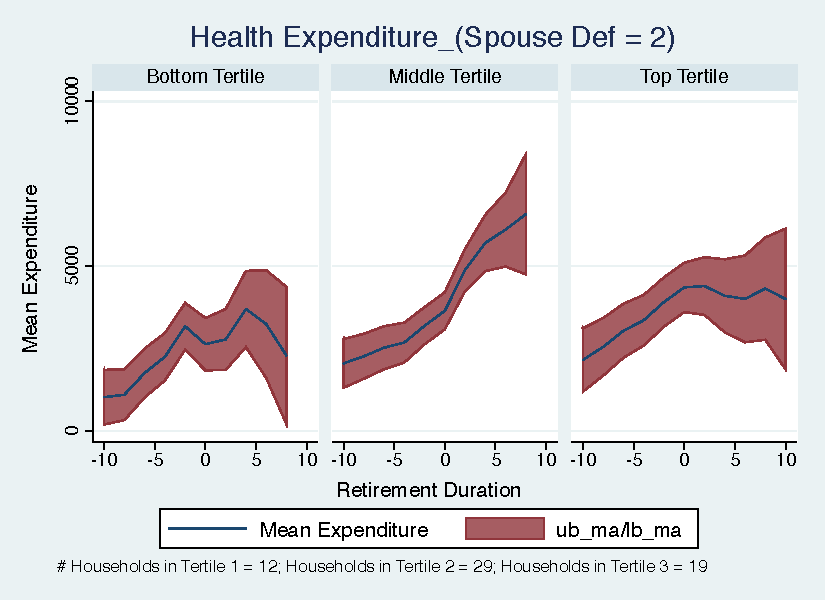
\includegraphics[width=0.6\textwidth]{../ConsumptionPostRetirement_by_SpouseDef_Cats/Smoothed/2/spouse_def_total_healthexpense_real.pdf}
\end{figure}


\begin{figure}[h]
	\caption{Expenditure on Non-Durable Transport}
	\centering
	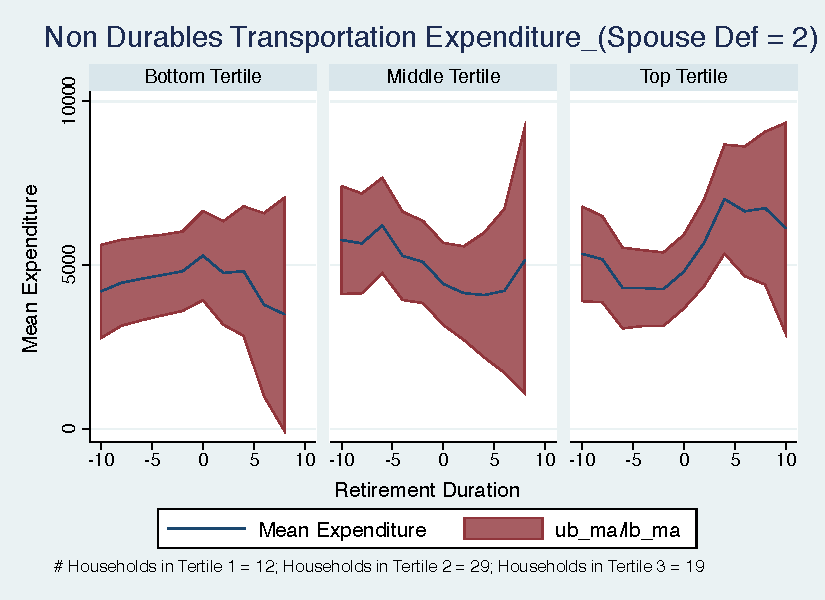
\includegraphics[width=0.6\textwidth]{../ConsumptionPostRetirement_by_SpouseDef_Cats/Smoothed/2/spouse_def_total_transport_real.pdf}
\end{figure}
\clearpage


\subsection{3- Spouse has same retirement transition +/- wave}

\begin{figure}[h]
	\caption{Food Expenditure at Home}
	\centering
	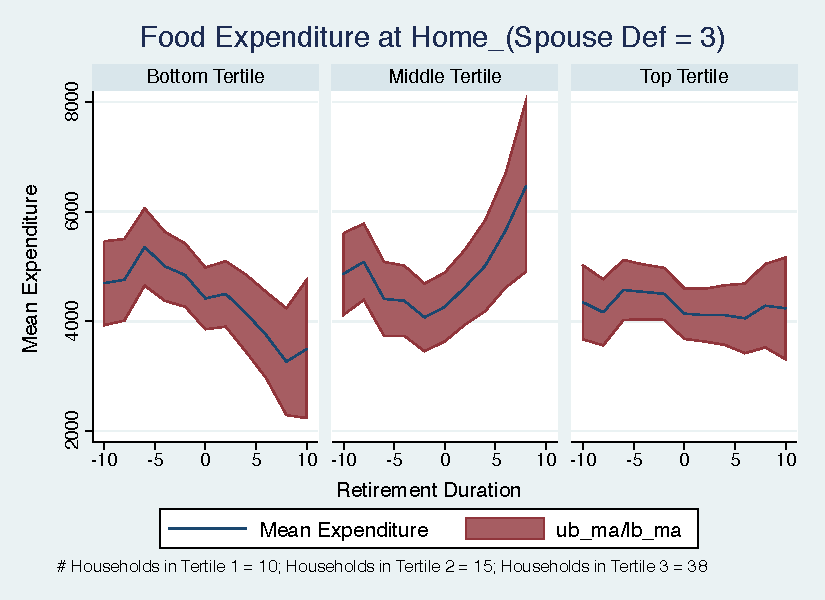
\includegraphics[width=0.6\textwidth]{../ConsumptionPostRetirement_by_SpouseDef_Cats/Smoothed/3/spouse_def_total_foodexp_home_real.pdf}
\end{figure}


\begin{figure}[h]
	\caption{Food Expenditure Away from Home}
	\centering
	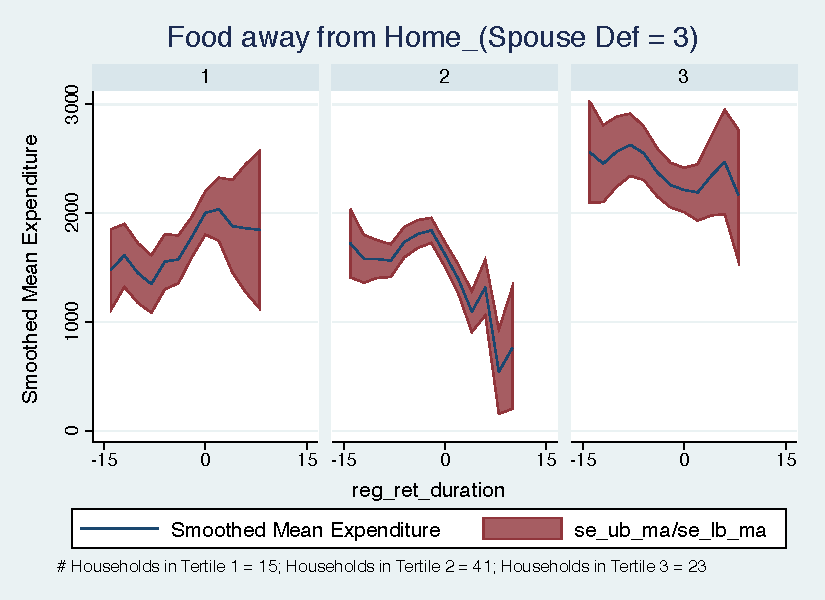
\includegraphics[width=0.6\textwidth]{../ConsumptionPostRetirement_by_SpouseDef_Cats/Smoothed/3/spouse_def_total_foodexp_away_real.pdf}
\end{figure}

\clearpage

\begin{figure}[h]
	\caption{Expenditure on Housing}
	\centering
	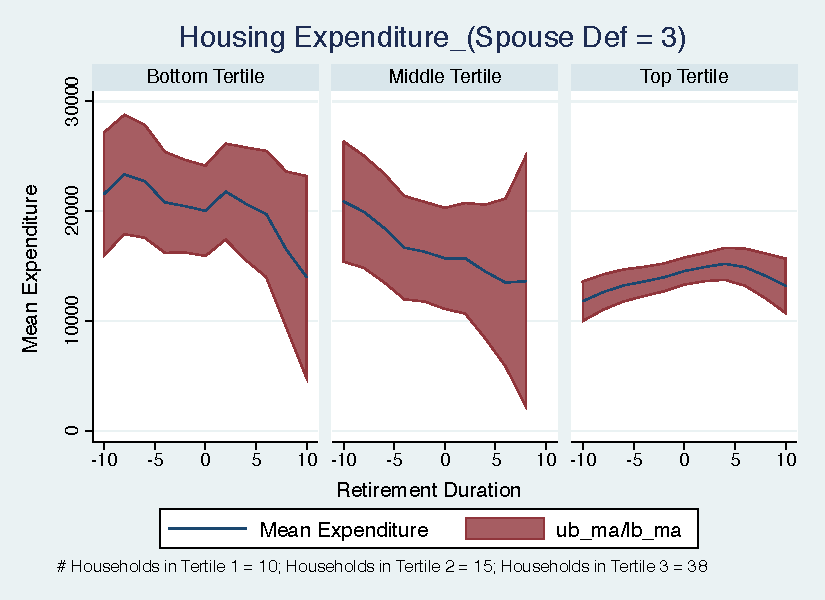
\includegraphics[width=0.6\textwidth]{../ConsumptionPostRetirement_by_SpouseDef_Cats/Smoothed/3/spouse_def_total_housing_real.pdf}
\end{figure}


\begin{figure}[h]
	\caption{Expenditure on Education}
	\centering
	\includegraphics[width=0.6\textwidth]{../ConsumptionPostRetirement_by_SpouseDef_Cats/Smoothed/3/spouse_def_total_education_real.pdf}
\end{figure}
\clearpage

\begin{figure}[h]
	\caption{Expenditure on Health}
	\centering
	\includegraphics[width=0.6\textwidth]{../ConsumptionPostRetirement_by_SpouseDef_Cats/Smoothed/3/spouse_def_total_healthexpense_real.pdf}
\end{figure}


\begin{figure}[h]
	\caption{Expenditure on Non-Durable Transport}
	\centering
	\includegraphics[width=0.6\textwidth]{../ConsumptionPostRetirement_by_SpouseDef_Cats/Smoothed/3/spouse_def_total_transport_real.pdf}
\end{figure}
\clearpage


\subsection{4-Spouse has Different Retirement Transition}

\begin{figure}[h]
	\caption{Food Expenditure at Home}
	\centering
	\includegraphics[width=0.6\textwidth]{../ConsumptionPostRetirement_by_SpouseDef_Cats/Smoothed/4/spouse_def_total_foodexp_home_real.pdf}
\end{figure}


\begin{figure}[h]
	\caption{Food Expenditure Away from Home}
	\centering
	\includegraphics[width=0.6\textwidth]{../ConsumptionPostRetirement_by_SpouseDef_Cats/Smoothed/4/spouse_def_total_foodexp_away_real.pdf}
\end{figure}

\clearpage

\begin{figure}[h]
	\caption{Expenditure on Housing}
	\centering
	\includegraphics[width=0.6\textwidth]{../ConsumptionPostRetirement_by_SpouseDef_Cats/Smoothed/4/spouse_def_total_housing_real.pdf}
\end{figure}


\begin{figure}[h]
	\caption{Expenditure on Education}
	\centering
	\includegraphics[width=0.6\textwidth]{../ConsumptionPostRetirement_by_SpouseDef_Cats/Smoothed/3/spouse_def_total_education_real.pdf}
\end{figure}
\clearpage

\begin{figure}[h]
	\caption{Expenditure on Health}
	\centering
	\includegraphics[width=0.6\textwidth]{../ConsumptionPostRetirement_by_SpouseDef_Cats/Smoothed/4/spouse_def_total_healthexpense_real.pdf}
\end{figure}


\begin{figure}[h]
	\caption{Expenditure on Non-Durable Transport}
	\centering
	\includegraphics[width=0.6\textwidth]{../ConsumptionPostRetirement_by_SpouseDef_Cats/Smoothed/4/spouse_def_total_transport_real.pdf}
\end{figure}
\clearpage

\subsection{5-Ignoring the spouse}

\begin{figure}[h]
	\caption{Food Expenditure at Home}
	\centering
	\includegraphics[width=0.6\textwidth]{../ConsumptionPostRetirement_by_SpouseDef_Cats/Smoothed/5/spouse_def_total_foodexp_home_real.pdf}
\end{figure}


\begin{figure}[h]
	\caption{Food Expenditure Away from Home}
	\centering
	\includegraphics[width=0.6\textwidth]{../ConsumptionPostRetirement_by_SpouseDef_Cats/Smoothed/5/spouse_def_total_foodexp_away_real.pdf}
\end{figure}

\clearpage

\begin{figure}[h]
	\caption{Expenditure on Housing}
	\centering
	\includegraphics[width=0.6\textwidth]{../ConsumptionPostRetirement_by_SpouseDef_Cats/Smoothed/5/spouse_def_total_housing_real.pdf}
\end{figure}


\begin{figure}[h]
	\caption{Expenditure on Education}
	\centering
	\includegraphics[width=0.6\textwidth]{../ConsumptionPostRetirement_by_SpouseDef_Cats/Smoothed/5/spouse_def_total_education_real.pdf}
\end{figure}
\clearpage

\begin{figure}[h]
	\caption{Expenditure on Health}
	\centering
	\includegraphics[width=0.6\textwidth]{../ConsumptionPostRetirement_by_SpouseDef_Cats/Smoothed/5/spouse_def_total_healthexpense_real.pdf}
\end{figure}


\begin{figure}[h]
	\caption{Expenditure on Non-Durable Transport}
	\centering
	\includegraphics[width=0.6\textwidth]{../ConsumptionPostRetirement_by_SpouseDef_Cats/Smoothed/5/spouse_def_total_transport_real.pdf}
\end{figure}
\clearpage

\section{testing}

\input{../Regression_Table/test.tex}

\end{document}

              